
%D�finir le format du document: papier, taille de police, type de document, etc.
\documentclass[a4paper, 11pt]{article}

%%%%%%%%% Packages externes utilis�s %%%%%%%%%%%%%%%%%%%
\usepackage[utf8]{inputenc}
\usepackage[french]{babel}
\usepackage[latin1]{inputenc}
\usepackage[T1]{fontenc}
\usepackage{verbatim}
\usepackage{graphicx}
\usepackage{epstopdf}

\usepackage{geometry}
 \geometry{
 [a4paper,
 total={210mm,297mm},
 left=20mm,
 right=20mm,
 top=20mm,
 bottom=20mm]
 }

%%%%%%%%% Le corps du document entre begin et end %%%%%%%%%%%%%%%%%%%
\begin{document}

%Page de garde
%%%%%%%%%%%%%%% Page de garde %%%%%%%%%%%%%%%%%%%

\begin{titlepage}{
    \begin{center}
        \vspace* {30mm}
        {\Large \textbf {Université de Cergy-Pontoise}} \\
        \vspace* {15mm}
        {\Large \textbf {RAPPORT}} \\
        \vspace* {15mm}
        pour le projet Génie Logiciel \\
        \textbf {Licence Informatique 2ème année} \\
        \vspace* {15mm}

	sur le sujet \\
        \vspace* {15mm}
	{\Huge \textsf{GARDIEN DE PARC}} \\
        \vspace* {10mm}
 	rédigé par \\
        \vspace* {10mm}
        \Large{} \textbf {} Makoura Karabouali, Antoine Phetramphand, \\Ramatoulaye Tangara\\
        \vspace* {10mm}
        \date \\ Mai 2014
        \vspace* {10mm}
	\end{center}
}
\end{titlepage}


%G�n�ration automatique de la table des mati�res, de la liste des figures et de la liste des tableaux
\tableofcontents
\listoffigures
\listoftables


\section{Introduction}
\label{sec:introduction}

\subsection{Les Fonctionnalités}
\begin{itemize}
\item Présenter au joueur une interface d’entrée dans le jeu
\item Mettre en évidence des éléments importants de la scène en les surlignant
\item Offrir une simplicité d'utilisation
\item Offrir une rapidité de mise en oeuvre
\item Assurer des temps d'exécution faibles
\item Assurer des temps d'interactions joueur / machine faibles
\end{itemize}

\subsection{Outils de développement}
\begin{enumerate}
\item Java
\item Eclipse
\item Latex
\end{enumerate}

\newpage

\section{Présentation du projet}
\label{sec:Présentation du projet}


    \subsection{sujet 4 :} le gardien de parc
		

\subsection{ Contexte}
\label{sec:spec1}
\paragraph{}L’intelligence artificielle est de plus en plus utilisée dans le monde d’aujourd’hui. Le
multi-agents réactifs est une méthode de programmation pour créer des intelligences artificielles.
Dans le cadre de notre formation à l’Université de Cergy Pontoise, les étudiants en Licence informatique deuxième année réalisent des projets personnels afin de valider leur année scolaire. Ce type de réalisation exige donc un certain temps, un investissement personnel et l’usage de toutes les ressources disponibles. Ici, nous allons réaliser notre projet sous la forme d’un jeu vidéo  appelé « le gardien de parc».

\subsection{ Objet}

\label{sec:spec2}
\paragraph{}Le but est la réalisation d’une application qui consiste à créer  un jeu qui permet de chasser les intrus  dans un espace  donné et de les éliminer.
  
\subsection{ Organisation}
\label{sec:spec3}
 \paragraph{}}Notre équipe est composée de trois membres à la charge du projet : Karabouali Makoura
, Phetramphand Antoine et Tangara Ramatoulaye. 
Pour mieux appréhender le projet, nous allons entamer des recherches et approfondir les non acquis et mettre le problème en œuvre techniquement en utilisant le processus «modèle en cascade». Il s'agit du modèle le plus simple des processus logiciels en termes de complexité et de facilité de mise en œuvre et repose sur les étapes suivantes :
		
		
\subsubsection{analyse}
\label{sec:spec1}
\paragraph{}On essaye de comprendre le problème ,puis d'analyser les besoins fonctionnels (contrainte technique).

\subsubsection{spécification}
\label{sec:spec2}
\paragraph{}On décrit les besoins du client, puis on traduit les besoins en fonctionnalités.

\subsubsection{conception}
\label{sec:spec3}
\paragraph{}On transforme le problème en solution.

\subsubsection{programmation}
\label{sec:spec4}
\paragraph{}On passe du résultat de la conception à un ensemble de programmes traduit en un langage de programmation ( Écriture des textes des programmes).

\subsubsection{tests}
\label{sec:spec5}
\paragraph{}On recherche des erreurs dans une spécification ou programme.

\subsubsection{validation}
\label{sec:spec6}
\paragraph{}Le système répond aux exigences du client et s'assure de l’adéquation des résultats de l'analyse et de la spécification.

\subsubsection{maintenance}
\label{sec:spec7}
\paragraph{}On veille au bon fonctionnement des programmes du projet.


\subsection{Environnement}
\label{sec:spec4}
\paragraph{}Les ressources  que nous disposons pour le développement de notre projet sont : 
\paragraph{Éclipse}:  un logiciel de développement. Son objectif est de produire et fournir des outils pour la réalisation de logiciels, englobant les activités de programmation permettant de réaliser notre projet en utilisant le langage Java.
\paragraph{SVN }: Subversion est un logiciel de gestion permettant de stocker , partager des fichiers texte informatique, et dispose d'un mécanisme intelligent de fusion des modifications apportées. C'est un outil très utilisé pour le développement de logiciels. 
\paragraph{Latex}: c'est un système de production de documents. Il ne s’agit pas de composer son texte, mais il s’agit d’utiliser un jeu de commandes décrivant ce que l’on souhaite obtenir.
 

\subsection{Plannification}
\label{sec:spec5}
\begin{figure}[h]
  \centering
  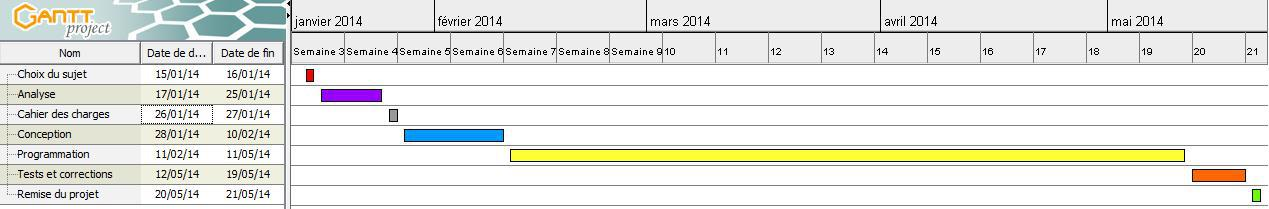
\includegraphics[width=500 , height=300]{images/planing.jpg}
  \caption{planning}
\end{figure}

\newpage

\section{Objectif}
\label{sec:Objectif}

\paragraph{} Nous avons présenté l'objectif du projet dans la section \ref{sec:introduction}. Dans cette section, nous présentons la spécification de notre logiciel réalisé. Ceci correspond principalement au cahier des charges.

\subsection{Description brève du logiciel}
\label{sec:spec1}
\paragraph{}L’objectif du projet consiste à développer un jeu ou une application basé sur un système de type «multi-agents réactifs» mettant en place comme éléments : un gardien, des intrus et des éléments du décor ou de l’interface graphique (eau, arbre, mur…).

\subsection{Le but du jeu}
\label{sec:spec2}
\paragraph{}Cela consiste à l’utilisateur à prendre en main un gardien qui a pour but d’attraper les intrus présents dans un environnement donné (ici un parc). L’idée est divertir l’utilisateur afin qu’il soit immergé dans le cadre du divertissement.

\subsection{Liste des fonctionnalités}
\label{sec:spec3}
\paragraph{}Cette application permettra de réaliser les fonctionnalités suivantes
\paragraph{Présenter au joueur une interface d’entrée dans le jeu}: cette interface expliquera à l’utilisateur la tâche qu’il devra accomplir.
\paragraph{- Mettre en évidence des éléments importants de la scène en les surlignant}l’utilisateur sera donc guidé implicitement.
\paragraph{- Offrir une simplicité d'utilisation }: le jeu devra être facile à utiliser et à manipuler.
\paragraph{- Offrir une rapidité de mise en œuvre}: le jeu doit permettre à des joueurs de mesurer leurs réflexes mentaux afin qu’il puisse prendre des décisions le plus rapidement possible lors de la partie du jeu.
\paragraph{- Assurer des temps d'exécution faibles }: lors du lancement du logiciel, les temps de chargement des programmes doivent être rapides.
\paragraph{- Assurer des temps d'interactions joueur / machine faibles }: durant l’exécution du logiciel, l’utilisateur ne doit sentir aucune latence, que ce soit avec le clavier ou la souris. Les déplacements du joueur doivent être fluides.

\subsection{Contraintes}
\label{sec:spec4}
\paragraph{}- Problème de repérage des intrus par le gardien lié a son champ de vision limité.\\
- Détermination de la position des intrus\\
- Présence de multiple intrus dans l'espace.\\
- Déplacements et simulation des intrus.\\

\newpage 

\section{Livraisons attendues}
\label{sec:Livraisons}
\paragraphe{}À la fin de notre projet, nous pensons rendre les documents suivants :
\begin{itemize}
  \item des programmes en langage java comportant une interface graphique  
  \item l’exécutable jar des programmes
  \item manuel d'utilisation  du logiciel
  \item un rapport
  \item un cahier des charges final
	\item un planning (en cours)
  \item javadoc
\end{itemize}

\newpage
\input{livraison.tex}\newpage


\section{Conception}
\label{sec:conception}

\paragraphe{}Voici notre diagramme de classes ci-dessous :

\begin{figure}
  \centering
  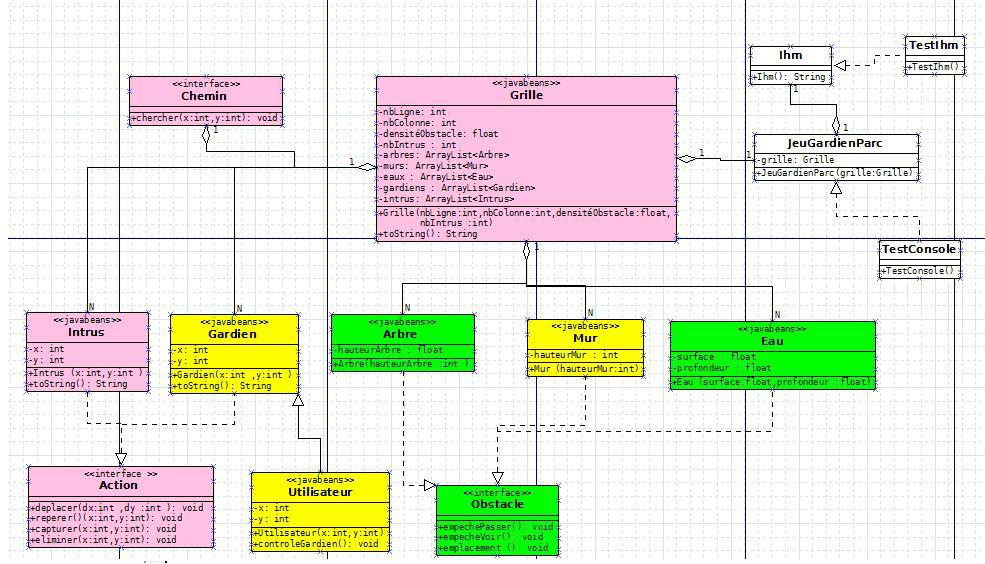
\includegraphics[width=500 ,height=300]{images/uml.jpg}
 
\end{figure}
\end{section}


\section{Manuel Utilisateur}
\label{sec:manuel}

\noindent Dans cette section, le manuel utilisateur du logiciel est présenté de façon concise.

\paragraph{} Tout d'abord, appuyer sur le bouton Commencez pour démarrrer l'application, attendez le chargement du jeu
\begin{enumerate}
\item Java
\item Eclipse
\item Latex
\end{enumerate}



%R�f�rences bibliographiques du document
\bibliographystyle{plain}
\bibliography{bibliographies}
\nocite{*}

\end{document}
